
\begin{flushleft}
	\bigskip
	\begin{figure}[h!]
		\centering
		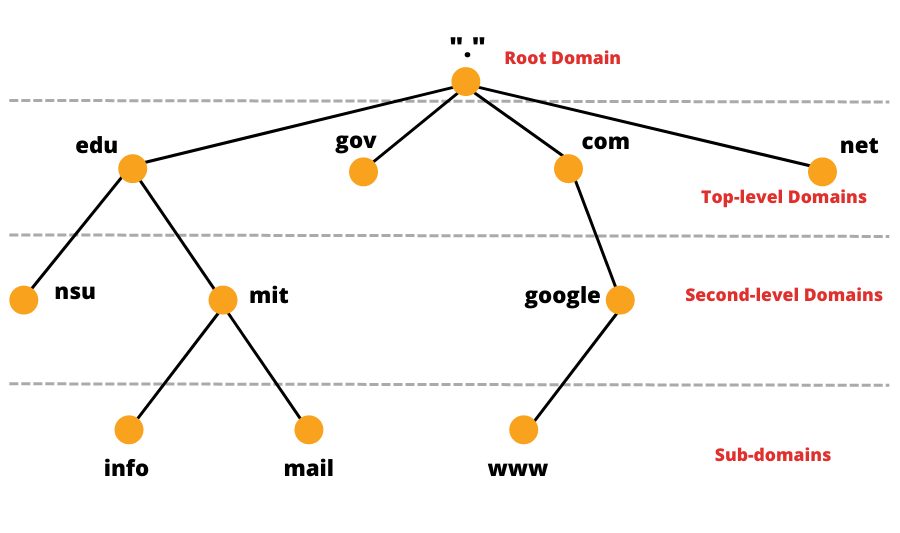
\includegraphics[scale=.6]{content/chapter3/images/dns.png}
		\caption{DNS Hierarchy}
		\label{fig:dns_heir}
	\end{figure}
	\begin{itemize}
		\item \textbf{What is domain?}
		\begin{itemize}
			\item A domain name is an easy-to-remember address used to access websites. 
		\end{itemize}
		\item A domain consist of:
		\begin{itemize}
			\item The \textbf{root-level domain} at the top
			\item The \textbf{top-level domains}(TLD) underneath it
			\item Followed by \textbf{second-level domains}
			\item Finally \textbf{sub-domains}.
		\end{itemize}
		Let's see each of these in detail

		\newpage
		
		
		\item \textbf{What is root-level domain?}
		\bigskip
		\begin{itemize}
			\item Root domain is the highest hierarchical level of the Internet.
			\bigskip
			\item When any DNS server is asked for an information which it does not have, the first thing that DNS server does is asking one of the (.)root name server.
			\begin{figure}[h!]
				\centering
				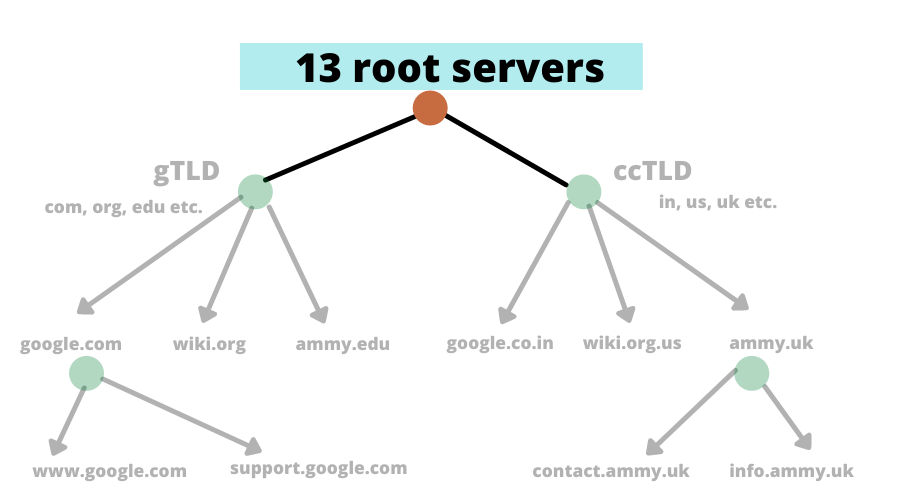
\includegraphics[scale=.5]{content/chapter3/images/page1.png}
				\caption{13 root servers}
				\label{fig:root_servers}
			\end{figure}		
			\item There are 13 root name servers as follows:
			\begin{itemize}
				\item a.root-servers.net.
				\item b.root-servers.net.
				\item c.root-servers.net.
				\item d.root-servers.net.
				\item e.root-servers.net.
				\item f.root-servers.net.
				\item g.root-servers.net.
				\item h.root-servers.net.
				\item i.root-servers.net.
				\item j.root-servers.net.
				\item k.root-servers.net.
				\item l.root-servers.net.
				\item m.root-servers.net.
			\end{itemize}
		\end{itemize}
		\newpage
		
			
		
		\newpage
		\item \textbf{What is TLD?}
		\bigskip
		\begin{itemize}
			\item TLDs tell users the general purpose of the service behind the domain name. 
			\bigskip
			\item Types of TLD:
			\begin{itemize}
				\item Generic TLDs (gTLDs) like \textbf{.com}, \textbf{.edu}, \textbf{.net}, etc.
				\item Country code TLDs (ccTLDs) like \textbf{.us}, \textbf{.uk}, \textbf{.ru}, \textbf{.in}, etc. 
			\end{itemize}  
		
			\begin{figure}[h!]
				\centering
				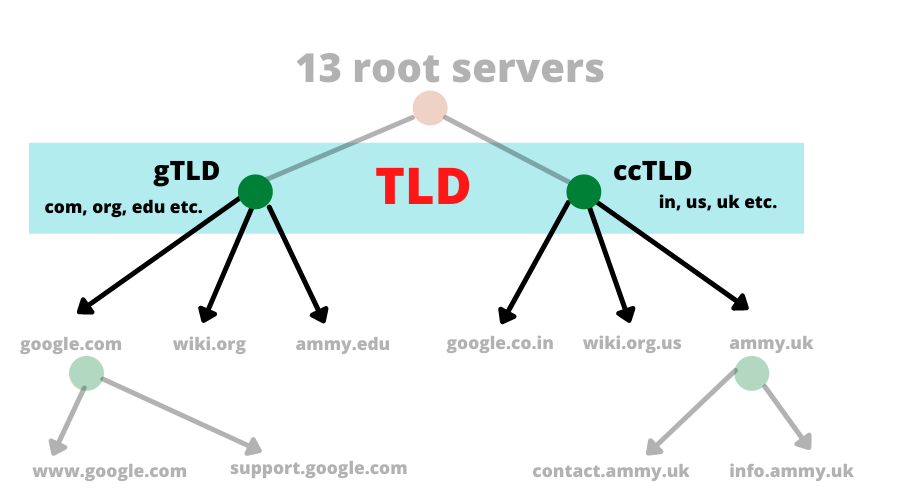
\includegraphics[scale=.5]{content/chapter3/images/page2.png}
				\caption{TLD types}
				\label{fig:tld}
			\end{figure}		
			\bigskip
			\item List of TLDs: https://data.iana.org/TLD/tlds-alpha-by-domain.txt
		\end{itemize}

		\newpage
		\item \textbf{What is second level domain?}
		\bigskip
		
		\begin{itemize}
			\item This is where domain holders put the brand name, project name, organization name or other familiar identifier for users.
			
			\begin{figure}[h!]
				\centering
				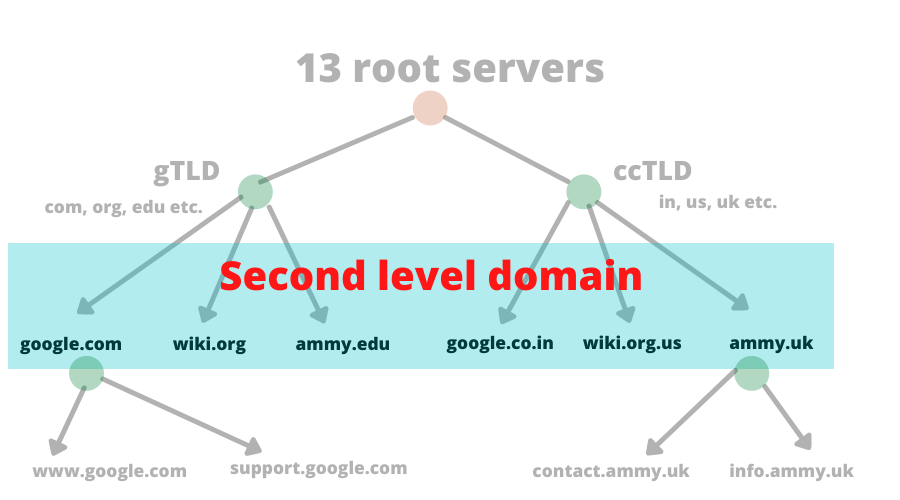
\includegraphics[scale=.5]{content/chapter3/images/page3.png}
				\caption{Second level domain}
				\label{fig:sec_domain}
			\end{figure}		
			
			\item Eg: For amazon.com, \textbf{amazon} is second level domain.
		\end{itemize}
	
		\newpage		
		\item \textbf{What is subdomain?}
		\bigskip
		\begin{itemize}
			\item It is additional information added to the front of website's domain name. 
			\bigskip
			\item It organizes the content for website.
			
			\begin{figure}[h!]
				\centering
				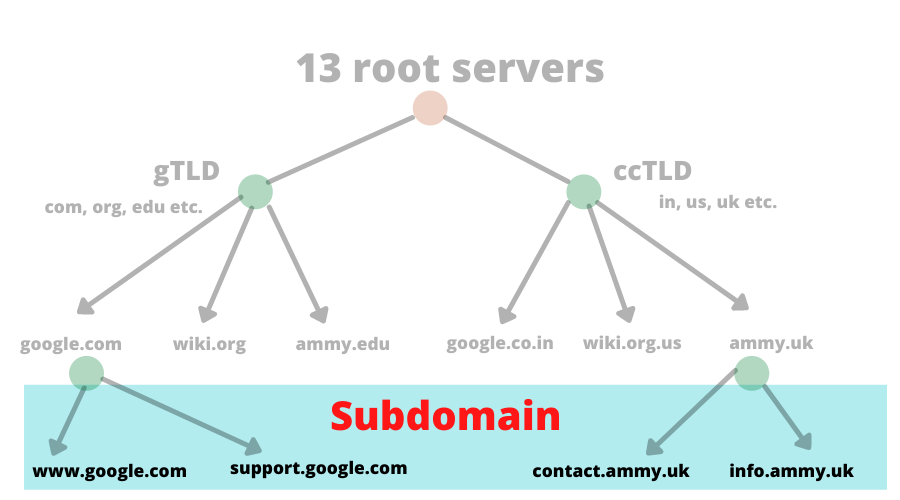
\includegraphics[scale=.5]{content/chapter3/images/page4.png}
				\caption{Subdomain}
				\label{fig:subdomain}
			\end{figure}		
							
		\end{itemize}
	
		\newpage
		
		\paragraph{Command examining the DNS query structure}
		\bigskip
		\item \textbf{dig +trace domainname}: Understand the entire flow of the query.
		\bigskip
		\begin{tcolorbox}[breakable,notitle,boxrule=-0pt,colback=black,colframe=black]
			\color{green}
			\fontdimen2\font=1em
			\# dig +trace google.com
			\fontdimen2\font=4pt
		\end{tcolorbox}
		Eg:
		\begin{figure}[h!]
			\centering
			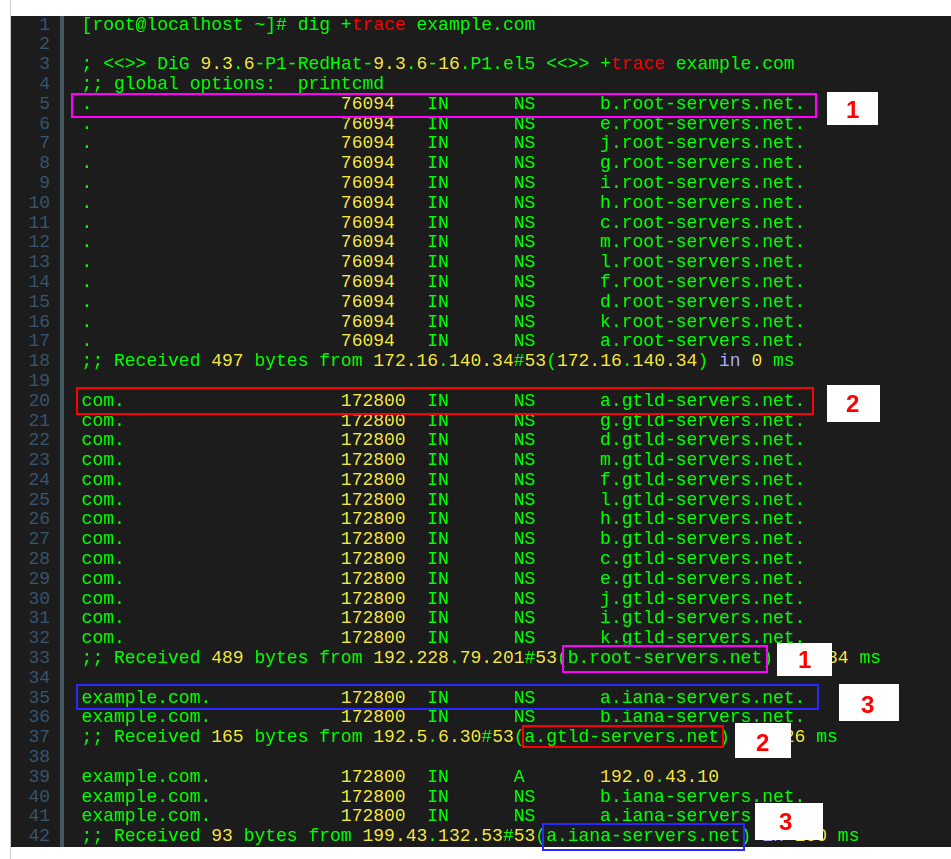
\includegraphics[scale=.35]{content/chapter3/images/dig.png}
			\caption{dig command output}
			\label{fig:dig}
		\end{figure}
		
		Understanding dig command output:
		\begin{itemize}
			\item \textbf{/etc/resolv.conf}: Your local dns server (in \textbf{/etc/resolv.conf}), provides with address of the \textbf{13 dns root servers}. 
			\item \textbf{Box 1}: Dig command selects one root server from the 13, to fetch the address of the \textbf{.com TLD servers}. 
			\item \textbf{Box 2}: The root server selected will reply with the \textbf{.com TLD server} addresses.
			\item \textbf{Box 3}: The \textbf{COM GTLD server} replied with IP address of "example.com" which is \textbf{192.0.43.10}.
			
			
		\end{itemize}
		
		
		

	\end{itemize}	
	
\end{flushleft}

\newpage
